\documentclass{article}
%\usepackage{lgrind}
\usepackage{graphicx}
\usepackage{verbatim}

\usepackage[font=small,labelfont=bf]{caption}

\pagestyle{plain}
\bibliographystyle{apalike}

\begin{document}

% TODO cover w/signatures?

\pagestyle{plain}
\title{Detecting Photo Manipulation using Reflections on Curved Surfaces}
\author{Laura A. Moss}
\date{}
\maketitle

\newpage

\subsection*{Abstract}
Abstract goes here
  % -*- Mode:TeX -*-
%% This file simply contains the commands that actually generate the table of
%% contents and lists of figures and tables.  You can omit any or all of
%% these files by simply taking out the appropriate command.  For more
%% information on these files, see appendix C.3.3 of the LaTeX manual. 
\tableofcontents
%\newpage
%\listoffigures
%\newpage
%\listoftables


% Body
\chapter{Introduction}

% TODO cases of forged images in journalism and science?

% TODO how long has the field been around?

% TODO examples of research


Image forensics, the study of finding hidden information in photographs, is an emerging field with diverse applications. It is comprised of a few general subtopics: determining the source of an image, detecting forgery, and detecting steganography (hiding information in a digital image) \cite{rocha2011}. All too often, pictures are used as hard evidence in journalism, scientific research, and criminal cases. For example, there was one incident in the scientific community in which a group of South Korean scientists published groundbreaking stem cell research results, but it was later revealed that the majority of the photographs included with the results were doctored \cite{rocha2011}. Image forgery itself predates the digital age, but as computers have become more capable and tools such as Adobe Photoshop have been developed, it has become much easier to manipulate images in a convincing manner. Therefore, there is an increasing need for forensic techniques as the technology develops.

Existing forensic techniques generally involve machine learning, finding statistical anomalies, or finding geometric inconsistencies. The current techniques that take advantage of reflective objects in an image fall into the latter category. Interestingly, the human eye is very insensitive to inconsistencies in reflections \cite{farid2010image}. Therefore it would be fairly straightforward for a forger to, for example, convincingly show a person in a scene with a reflective surface who was never actually there. It would perhaps be convincing to a human, but may not hold up to analysis with a geometric technique.

Most of the reflective surfaces that might be found in real photos are planar. Some common examples are bodies of still water, mirrors, and glass windows. Non-planar reflective surfaces, which are the focus of this paper, are less common but can be found in the form of store security mirrors, works of art, and even the human eye.

\section{Prior Work}
\subsection{Reflections on Planar Surfaces}
% TODO where and how to cite O'Brien/Farid paper
% Summary of planar reflections

\begin{figure}
	\centering
    	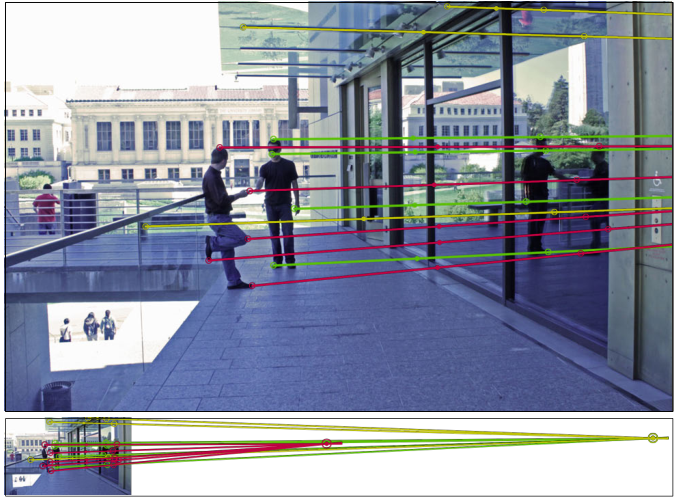
\includegraphics[width=0.8\textwidth]{planar-vanishing-point-forged}
	\caption{Demonstration of vanishing point inconsistency. The lines corresponding to the man on the left converge to a different vanishing point than those from the rest of the scene, so it is likely that the man and his reflection were edited into the scene. \cite{obrien12}}
	\label{planar-vanishing-point-forged}
\end{figure}

\begin{figure}
	\centering
    	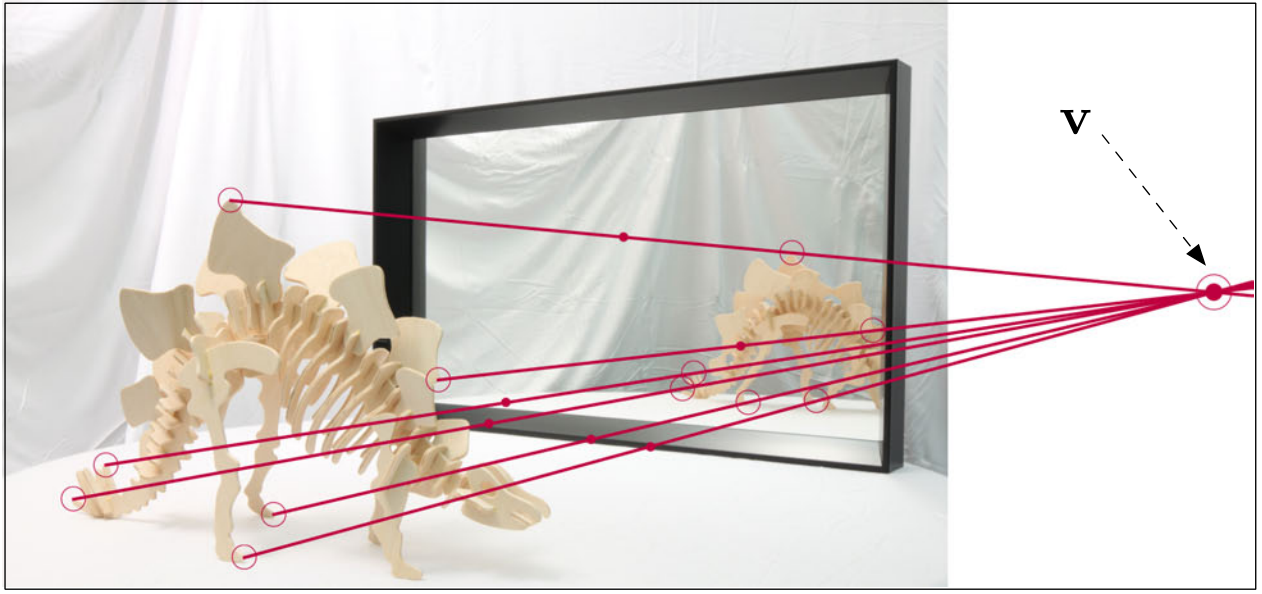
\includegraphics[width=0.8\textwidth]{planar-midpoint-genuine}
	\caption{Demonstration of midpoint and vanishing point consistency. The lines converge to a well-defined vanishing point $V$. Additionally, the midpoints in three-dimensional scene space between the real and reflected features plausibly intersect the mirror plane. \cite{obrien12}}
	\label{planar-midpoint-genuine}
\end{figure}

\begin{figure}
	\centering
    	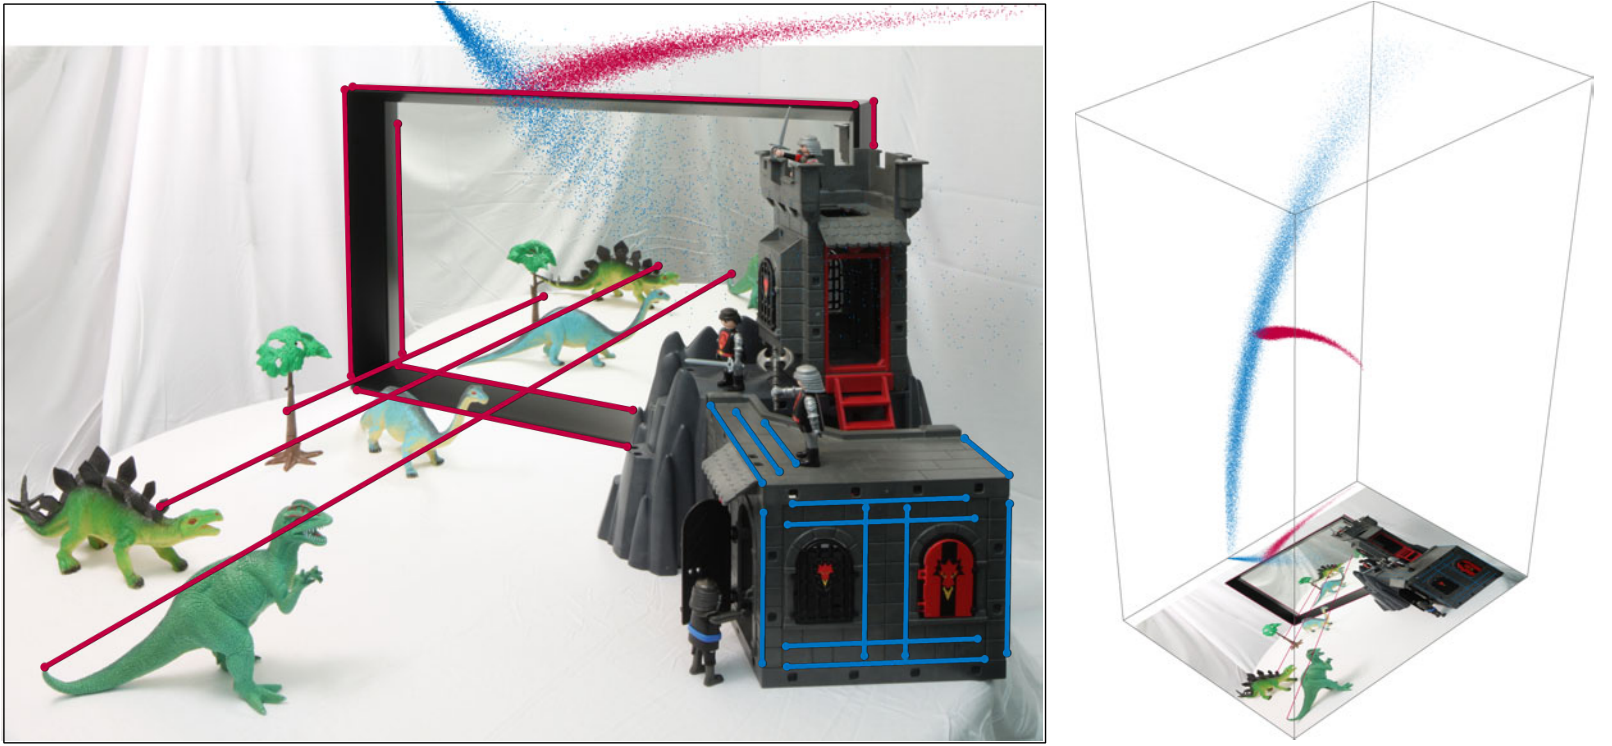
\includegraphics[width=0.8\textwidth]{center-of-projection-planar-genuine}
	\caption{Demonstration of center of projection consistency. The pink and blue point clouds represent sets of possible solutions, generated by randomly perturbing the points selected that form the lines. Since the point clouds intersect, there is a possible consistent center of projection, or camera position. \cite{obrien12}}
	\label{center-of-projection-planar-genuine}
\end{figure}

Recent research into properties of images that can be exploited to find inconsistencies has shown that an object in an image and its reflection in a mirror must have certain geometric properties in a real, unmanipulated image. O'Brien and Farid's 2012 paper discusses several techniques for determining whether or not an image that contains a planar mirror is consistent.\nocite{obrien12} All of these techniques are derived directly from linear perspective projection geometry.

The first step to all of the techniques is obtaining lines in the image that are parallel in three-dimensional scene space (or should be if the image is genuine). The first couple of techniques require hand-picking matching points between the original objects in the scene and their virtual (reflected) counterparts. Then, straight lines are drawn connecting these point pairs out to infinity. These lines, if drawn through the same planar mirror, must all intersect at a single vanishing point. If they don't intersect cleanly, or intersect at multiple vanishing points, the image can be assumed to be forged, as seen in Figure~\ref{planar-vanishing-point-forged}. Furthermore, the midpoints of the same lines, in three-dimensional scene space, must also plausibly appear to intersect the reflective surface, as in Figure~\ref{planar-midpoint-genuine}. Finally, as in Figure~\ref{center-of-projection-planar-genuine}, if there are orthogonal parallel lines in the image (for example, on the frame of a mirror), we can check if there is a consistent position for the center of projection, or point camera.


\subsection{Other Related Work}
Shadows

\section{Mathematical Techniques}
\subsection{Assumptions}
To simplify the geometry of this analysis, we will restrict the form of our non-planar mirrors to various types of quadric surfaces. This is likely to be good enough for typical use cases because most general curves encountered in the real world can be approximated as either a quadric surface or a set of quadric surfaces.

We also assume the camera used to take any of the images analyzed is a point camera, which is a reasonable assumption considering both the size of most digital camera sensors, and the fact that the camera would have to be far enough away from the subjects of the photograph to capture everything required to perform the analysis.
An important idea to note is that showing that an image is consistent according to these techniques is not sufficient to prove that the image is genuine, because the image could have had some counter-forensic techniques applied or been manipulated in a way that is unrelated to reflective geometry.

\subsection{Properties of Reflective Geometry}
% Will contain some more technical references to O'Brien/Farid paper where needed
Reflection of light on a surface is directly related to the surface normal at the point of reflection. The incident ray (or ray of light coming towards the surface) must make the same angle with the normal as the reflected ray.  Additionally, the incident ray, reflected ray, and normal must all be coplanar, and the reflected and incident rays must be on opposite sides of the normal.

\begin{figure}
	\centering
    	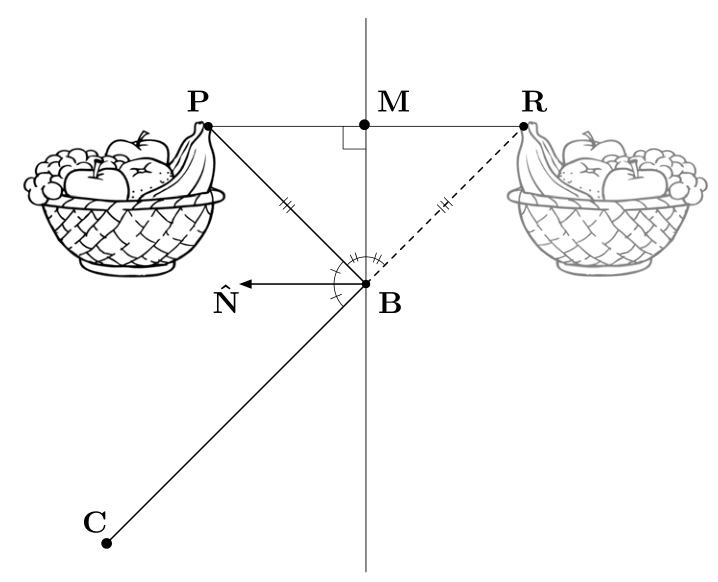
\includegraphics[width=0.6\textwidth]{normal-reflection}
	\caption{Given a camera location $C$, a point $P$ on an object and its corresponding reflection $R$, the ray $PR$ appears equivalent to the ray $PB$ from the point of view of the camera. The ray $PR$ is also perpendicular to the surface normal $N$. Since all of the points in this diagram must be coplanar, this holds true in 3D space. \cite{obrien12}}
	\label{normal-reflection}
\end{figure}

O'Brien and Farid point out that a non-obvious consequence of this law is that if a ray is drawn between the reflected object and its reflection, it should appear to be parallel to the surface normal at the point of reflection. (In the planar case, it would appear perpendicular to the mirror, since the normal is constant over the whole surface.) Furthermore, the ray drawn between the reflected object and its reflection, and the reflected object and its reflection point are the co-linear from the perspective of a point camera, as demonstrated in Figure~\ref{normal-reflection}. This is why drawing rays on a picture between an object and its reflection works: it appears equivalent to drawing rays to the apparent position of the reflected object. In the case of a planar mirror, all of these rays would be parallel in three-dimensional space.\nocite{obrien12} An axiom of linear perspective projection is that parallel lines projected onto a 2-D image must converge to some vanishing point $V$ \cite[p.~2]{hartley}, so all such lines through a planar mirror converge at a single vanishing point.

In the case of a curved surface, the ray is still parallel to the normal at the point of reflection. However, all such rays through the same mirror will not be parallel in three-dimensional space because the normal is not constant.
% relationship between normal and reflection angle
% colinearity of 3-D line between real and virtual object, and line between real object and reflection - why planar works
% still parallel to normal even if surface is curved


% TODO actual techniques

\section{Implementation}
In order to expedite the process of obtaining images that meet a variety of very specific conditions, all images used to test these algorithms were computer-generated using Blender 2.68a.

\subsection{Circle Finding}

\


\section{Conclusion}
\subsection{Results}
\subsection{Future Work}

\clearpage

\appendix
%\include{appa}
%\clearpage

\bibliography{Master}
\end{document}

